Database designet er en to delt affære. Der er selve strukturen i databasen også er der koden som tilgår databasen.
Disse beskrive begge i følgende afsnit.

\subsubsection{Database Opbygning}
Opbygning goes here.

\subsubsection{Database kode}
For at kunne tilgå databasen fra C\# blev det besluttet at bruge \gls{EF}. 
Det blev valgt at bruge "Code First from existing database" da designet af databasen var lavet i forvejen.
Ved at følge den fremgangsmåde bliver der lavet en model af databasen i form af objekter som \gls{EF} 
kan mappe til i figur \ref{fig:CodeFirstFromDB} er princippet illustreret.

\begin{figure}[H]
    \centering
	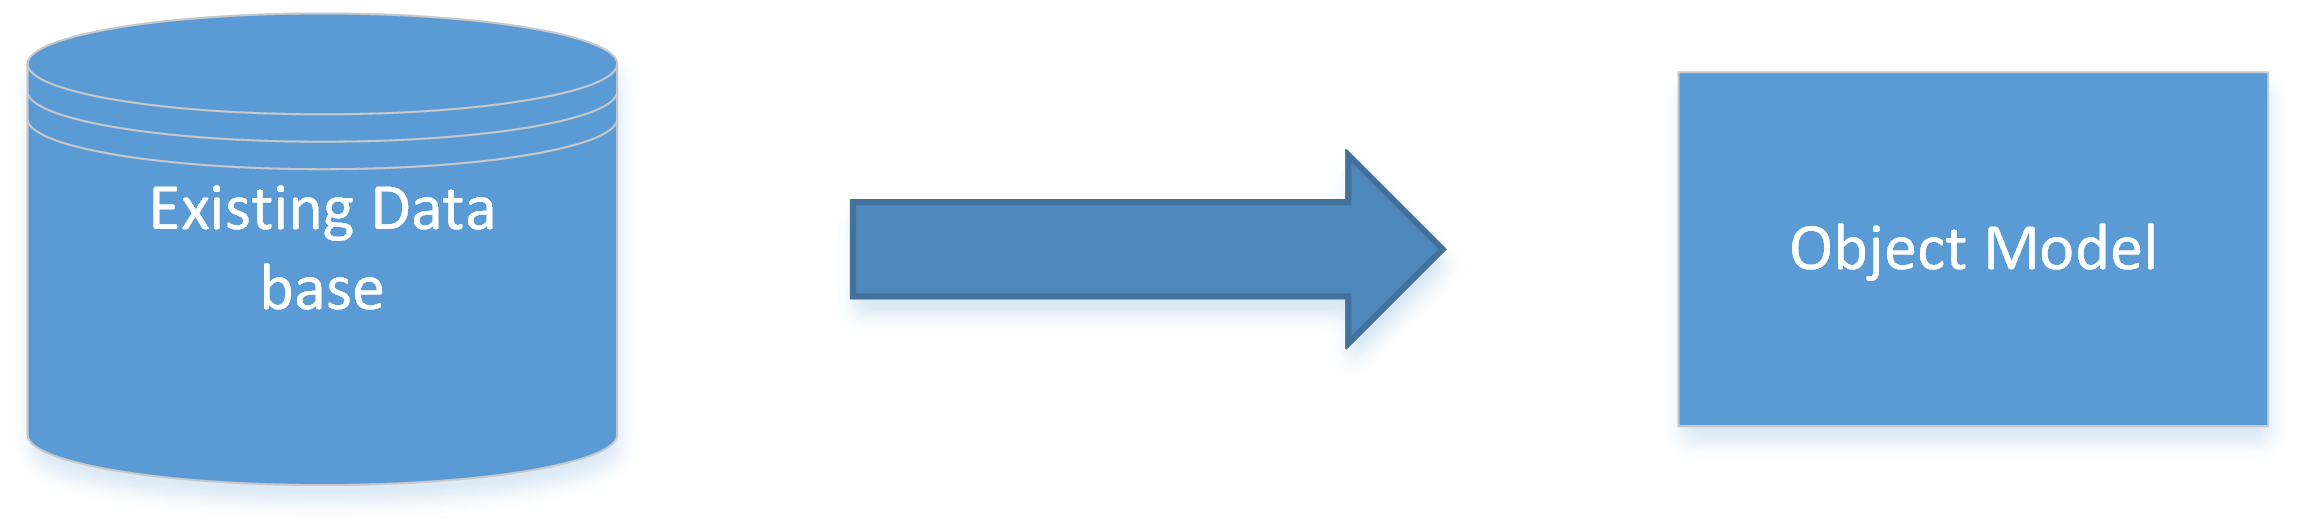
\includegraphics[scale=1]{Rapport/EFCFFDB.PNG}
	\caption{Skitse af GUI}
	\label{fig:CodeFirstFromDB}
\end{figure} 

Det virkede meget godt til første iteration af databasen, men herefter viste det sig at være lettere at få \gls{EF} til at bygge
databasen udfra koden ved ændringer.
\newline
Det blev også besluttet at pakke \gls{EF} ind i \gls{DAL} dette blev brugt for at skille framework koden fra vores program.
\gls{DAL} Består af tre klasser en Facade klasse, en Unitofwork klasse og en Repository klasse. 
Facaden er brugt til at sørge for at der kun findes et Unitofwork af gangen. 
Unitofwork er en samling af Repositorys, Unitofwork's opgave er at sørge for at der bliver kaldt "Save" på \gls{EF}'s context.
Repository er metoder til at udføre Create, Read, Update and Delete.
